\subsection{Prototype 2}

This prototype tries to answer \cref{rq:23}, \cref{rq:24}, \cref{rq:25} and \cref{rq:26}:
\begin{displayquote}
  How should the editor cooperate with multiple other tools that change the same underlying model?\\
  What data is required for displaying a model as a tree?\\
  How can a tree editor component be generic enough to support arbitrary user actions?\\
  How can the user interface know the model well enough so the user is constrained from creating invalid Ecore trees?
\end{displayquote}

\subsubsection{Requirements}

\paragraph*{Cooperation (\cref{rq:23})}
Cooperation in \cref{rq:23} could possibly be solved by channeling any model edits through a Model Server, and listening to this server for change notifications. An example of this was seen in \cref{sec:coffee-ide} with the \emph{Coffee Editor} reference implementation for \gls{GLSP} (\cref{sfig:coffee-example-glsp}).

\paragraph*{Tree model (\cref{rq:24})}
By displaying an example tree, the required data will be evident as the view is implemented.

\paragraph*{Generic actions (\cref{rq:25})}
By supporting actions through buttons in the user interface, but not hardcoding their clicks to trigger an action, they can be generic.
This means a click must only notify something that an \emph{intent} to trigger action \texttt{XYZ} has happened.
Implementing a skeleton for this would show what data is required for generic actions.

\paragraph*{Constrain tree for validity (\cref{rq:26})}
This is relevant especially for drag-and-drop, where a user should not be able to drop a node onto an ``incorrect'' parent.
Due to time constraints, drag-and-drop will not be implemented now.
But the supporting data structure could be sketched out, based on the previous data structures for the Tree model in \cref{rq:24}.

\paragraph*{Here is the list of identified requirements for this prototype:}

\begin{itemize}
  \item Develop using VSCode extension \acrshort{API} (see \cref{sec:vscode-extension}). No dependencies to Theia.
  \item Visualize a tree structure in the editor, based on a object structure (e.g. \gls{JSON}).
  \item Show labels and icons for nodes in the tree. Labels will be from node \emph{type}, labels from node data.
  \item Add and remove nodes in the tree from user interaction.
  \item Property sheet editor that is synchronized with tree selection.
  \item Visualize both an Ecore meta-model and model instance.
  \item Use EMF.Cloud Model Server (\cref{sec:model-server}) to get the model. Do not read the \texttt{.ecore} file from disk in the extension.
  \item Automatically update the views when the underlying model changes (push not poll)
\end{itemize}

The \textit{design document} used for implementation is added in \cref{app:prototype-2-design-doc}.

\subsubsection{Implementation}

\paragraph*{Setting up the project}
Similar to prototype 1, a new \gls{VSCode} Extension project was created.
A \emph{standalone} version of the EMF.Cloud Model Server (\cref{sec:model-server}) was downloaded\footnote{Snapshot builds are provided at sonatype: \href{https://oss.sonatype.org/content/repositories/snapshots/org/eclipse/emfcloud/modelserver/org.eclipse.emfcloud.modelserver.example/0.7.0-SNAPSHOT/}{https://oss.sonatype.org/content/repositories/snapshots/ org/eclipse/emfcloud/modelserver/org.eclipse.emfcloud.modelserver.example/0.7.0-SNAPSHOT/}.}
Unlike Coffee Editor IDE, this implementation does not use Theia Tree Editor (\cref{sec:theia-tree-editor}), because of its incompatibility with \gls{VSCode}.
A minimal, ``homemade'' solution was made instead, with CSS, HTML lists (\texttt{ol} and \texttt{li}) and some javascript.

\paragraph*{Connecting to VSCode APIs}
The editor had to use the \texttt{WebView} \acrshort{API}, being a non-text editor.
The javascript and CSS for a WebView exists in a separate folder without access to the rest of the extension code.
This is based on an official Microsoft tutorial called \emph{PawDraw}\footnote{\href{https://github.com/microsoft/vscode-extension-samples/tree/master/custom-editor-sample}{https://github.com/microsoft/vscode-extension-samples/tree/master/custom-editor-sample}.}.

The other piece of the puzzle was a \texttt{CustomDocument} and \texttt{CustomEditorProvider}.
These act as the glue between the \texttt{WebView}, VSCode and the extension.
Saving and file operations run through these \acrshortpl{API}.
Most of the handlers on \texttt{CustomEditorProvider} were left unimplemented, as only \texttt{resolveCustomEditor} was crucial.
This is the function that configures the \texttt{WebView} for the extension, providing it the tree editor HTML, javascript and CSS etc..

\paragraph*{The Tree Editor WebView}
Inside the \texttt{WebView} lives the actual editor user interface.
It has security restrictions when it comes to where resources (images etc.) can be loaded from.
To test a method for arbitrary icons, an image encoding called \emph{data-uri} was used.
It simply encodes the raw image to a Base64 string and prepends some metadata.
The result is one long string for one image.
A protocol could pass these images for tree node icons instead of referring to file paths.
A data structure mapped node types to an icon string, as seen in \cref{lst:prototype2-default-icons}.

\lstinputlisting[
    caption={Javascript code from the WebView to map icon graphics to tree node types.},
    label=lst:prototype2-default-icons,
    language=JavaScript
]{listings/default-icons.js}

To get the data for tree nodes, a sample data structure was created (see \cref{lst:prototype2-node-tree} for the data).
No real \gls{emf} or \gls{XMI} data was read in yet.
The fields in the structure were evolved alongside the tree view, adding or restructuring properties when issues arose.
A \texttt{name} was deemed essential for every node, and moved outside of the \texttt{properties}.
For determining the \emph{node types}, the \gls{Ecore} class name was used as the type.
(It is uncertain how this works with generics or inheritance, but I assume the type parameters and children could be mapped into the type value, e.g. by appending them).
Clicking on a node would store the node as the \emph{selected node}, and trigger an event listener (so the property sheet and action bar could update).

\lstinputlisting[
    caption={Javascript code from the WebView for a data model describing the tree nodes.},
    label=lst:prototype2-node-tree,
    language=JavaScript
]{listings/node-tree.js}

\paragraph*{Form based property editor}
A simple form was updated with the data of the selected tree node.
Changes were sent as notifications to VSCode.
These notifications only accept data that can be serialized to \gls{JSON}.
(The communication from the \texttt{WebView} to the \gls{VSCode} Extension \emph{could} possibly be made with \gls{JSON-RPC} in the future. It was not needed for now).

\paragraph*{Action bar}
An area with buttons was created to trigger arbitrary model actions, such as on-demand validation, genmodel code generation and dynamic instance creation.
The actions took their label from an action list, and every action has an \emph{id}. This is shown in \cref{lst:prototype2-action-list}.
Icons could be added in the same way, but was not done.
This abstracts actions to only id and label, and then the Tree Language Server could deal with the details of triggering the action.

\lstinputlisting[
    caption={Javascript code from the WebView to specify the available actions.},
    label=lst:prototype2-action-list,
    language=JavaScript
]{listings/available-actions.js}

A list specified which id to always show in the action bar.
Another data structure held mappings between node types and lists of actions.
This would allow different actions to be available based on the selected tree node. This is shown in \cref{lst:prototype2-action-schema}.

\lstinputlisting[
    caption={Javascript code from the WebView to specify default actions and per-node actions.},
    label=lst:prototype2-action-schema,
    language=JavaScript
]{listings/action-schema.js}


\paragraph*{Constraining the tree hierarchy}
No user manipulation of the tree was implemented, due to time constraints.
But a data structure that could identify which children are valid for a node type was specified.
This is shown in \cref{lst:prototype2-hierarchy-schema}.
The idea is to consult this mapping when deciding if a child node can be put into a specific parent node, which happens during drag-and-drop and copy-paste operation.


\lstinputlisting[
    caption={Javascript code from the WebView to specify what children a node type can have.},
    label=lst:prototype2-hierarchy-schema,
    language=JavaScript
]{listings/hierarchy-schema.js}


\paragraph*{Model Server}
The model server was only partially integrated, due to time constraints.
It was started manually, and only a single endpoint was used, which was selecting the \emph{model workspace directory}.
This is the directory where the Model Server will scan for \texttt{.ecore} and \texttt{.xmi} files.
The extension send a request to the Model Server's \gls{REST} \acrshortpl{API} with the workspace folder.
A testing command to create a new model file was also implemented.
This was a VSCode Command which prompted the user for a filename.
Then the extension would send the filename and an example EObject (serialized as \gls{JSON}) to the Model Server.
The Model Server would create a new \gls{XMI} file when receiving this request.


\subsubsection{Results}
The editor worked, but due to time constraints, some features were dropped.
Mainly user editing and model updates were not done, as well as automatic ecore-model-to-tree conversion.
A screenshot of the model is shown in \cref{fig:prototype-2-screenshot}.

\begin{figure}[htbp]
  \centering
  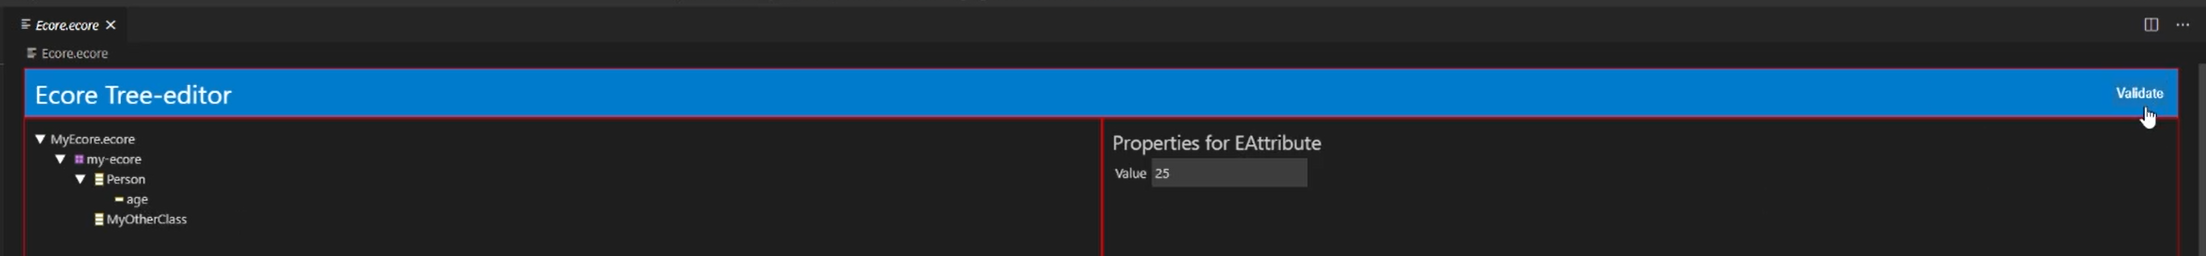
\includegraphics[width=\textwidth]{figures/prototype-2-screenshot.png}
  \caption[Prototype 2 Screenshot]{A screenshot of the prototype 2 in action. It has three parts: an action bar on the top right, a tree view on the left, and a property editor on the right.}\label{fig:prototype-2-screenshot}
\end{figure}

\paragraph*{Research questions}
The answer to \cref{rq:23} is:
\begin{displayquote}
  \emph{By reading the model data structure from a shared model server, and only editing it by using this model server.}
\end{displayquote}

The answer to \cref{rq:24} is:
\begin{displayquote}
  \emph{A nested datastructure of nodes, with labels and node types, as well as properties for each node. See \cref{lst:prototype2-node-tree} for an example.}
\end{displayquote}

The answer to \cref{rq:25} is:
\begin{displayquote}
  \emph{By only defining actions as id and label, and sending a schema of default actions and per-node actions to the frontend. Triggering an action will only send a message to the backend Tree Language Server, where this server executes any actual change. See \cref{lst:prototype2-action-list} and \cref{lst:prototype2-action-schema}} for examples.
\end{displayquote}

The answer to \cref{rq:26} is:
\begin{displayquote}
  \emph{By defining a parent-child schema based on node types, that specifies which children are allowed in a parent. See \cref{lst:prototype2-hierarchy-schema} for an example.}
\end{displayquote}
This last answer was not properly tested due to time constraints.